\newcommand{\lastversion}{0.1.0}%versione del documento
\newcommand{\doctitle}{Norme di progetto}%nome documento
\newcommand{\info}{\doctitle\ v\lastversion}
\begin{tiny}
{\tiny •}
\end{tiny}\begin{tiny}
•
\end{tiny}% In questo file vengono definiti comandi (macro) utili in tutti i documenti

\newcommand{\gruppo}{\textit{Sirius}} % nome gruppo
\newcommand{\progetto}{\textit{Sequenziatore}} % nome progetto
\newcommand{\capitolato}{\href{http://www.math.unipd.it/~tullio/IS-1/2013/Progetto/C4p.pdf}{http://www.math.unipd.it/~tullio/IS-1/2013/Progetto/C4p.pdf}} 

% GLOSSARIO
\newcommand{\lastversionG}{4.0.0}
\newcommand{\Glossario}{\textit{Glossario\_{}v\lastversionG{}.pdf}}
\newcommand{\doctitleG}{Glossario}
\newcommand{\infoG}{\doctitleG\ v\lastversionG}

% NORME DI PROGETTO
\newcommand{\lastversionNDP}{4.0.0}
\newcommand{\NormeDiProgetto}{\textit{NormeDiProgetto\_{}v\lastversionNDP{}.pdf}}
\newcommand{\doctitleNDP}{Norme di progetto}
\newcommand{\infoNDP}{\doctitleNDP\ v\lastversionNDP}

% ANALISI DEI REQUISITI
\newcommand{\lastversionAR}{3.0.0}
\newcommand{\AnalisiDeiRequisiti}{\textit{AnalisiDeiRequisiti\_{}v\lastversionAR{}.pdf}}
\newcommand{\doctitleAR}{Analisi dei requisiti}
\newcommand{\infoAR}{\doctitleAR\ v\lastversionAR}

% Studio di fattibilita
\newcommand{\lastversionSDF}{2.0.0}
\newcommand{\StudioDiFattibilita}{\textit{StudioDiFattibilita\_{}v\lastversionSDF{}.pdf}}
\newcommand{\doctitleSDF}{Studio Di Fattibilità}
\newcommand{\infoSDF}{\doctitleSDF\ v\lastversionSDF}

% Piano di qualifica
\newcommand{\lastversionPDQ}{4.0.0}
\newcommand{\PianoDiQualifica}{\textit{PianoDiQualifica\_{}v\lastversionPDQ{}.pdf}}
\newcommand{\doctitlePDQ}{Piano Di Qualifica}
\newcommand{\infoPDQ}{\doctitlePDQ\ v\lastversionPDQ}

% VERBALE 2014-02-03
\newcommand{\lastversionVb}{2.0.0}
\newcommand{\VerbaleB}{\textit{Verbale2014-02-03\_{}v\lastversionVb{}.pdf}}
\newcommand{\doctitleVb}{Verbale 2014-02-03}
\newcommand{\infoVb}{\doctitleVb\ v\lastversionVb}

% VERBALE 2014-07-20
\newcommand{\lastversionVN}{1.0.0}
\newcommand{\VerbaleN}{\textit{Verbale2014-07-20\_{}v\lastversionVN{}.pdf}}
\newcommand{\doctitleVN}{Verbale 2014-07-20}
\newcommand{\infoVN}{\doctitleVN\ v\lastversionVN}

%Piano di progetto
\newcommand{\lastversionPDP}{4.0.0}
\newcommand{\PianoDiProgetto}{\textit{PianoDiProgetto\_{}v\lastversionPDP{}.pdf}}
\newcommand{\doctitlePDP}{Piano Di Progetto}
\newcommand{\infoPDP}{\doctitlePDP\ v\lastversionPDP}
%Specifica Tecnica
\newcommand{\lastversionST}{3.0.0}
\newcommand{\SpecificaTecnica}{\textit{SpecificaTecnica\_{}v\lastversionST{}.pdf}}
\newcommand{\doctitleST}{Specifica Tecnica}
\newcommand{\infoST}{\doctitleST\ v\lastversionST}
%Definizione di prodotto
\newcommand{\lastversionDP}{2.0.0}
\newcommand{\DefinizioneDiProdotto}{\textit{DefinizioneDiProdotto\_{}v\lastversionDP{}.pdf}}
\newcommand{\doctitleDP}{Definizione Di Prodotto}
\newcommand{\infoDP}{\doctitleDP\ v\lastversionDP}

% MANUALE UTENTE
\newcommand{\lastversionMU}{2.0.0}
\newcommand{\ManualeUtente}{\textit{ManualeUtente\_{}v\lastversionMU{}.pdf}}
\newcommand{\doctitleMU}{Manuale utente}
\newcommand{\infoMU}{\doctitleMU\ v\lastversionMU}

% MANUALE PROCESS OWNER
\newcommand{\lastversionMPO}{2.0.0}
\newcommand{\ManualePO}{\textit{ManualeProcessOwner\_{}v\lastversionMPO{}.pdf}}
\newcommand{\doctitleMPO}{Manuale process owner}
\newcommand{\infoMPO}{\doctitleMPO\ v\lastversionMPO}% macro
\documentclass[11pt,a4paper]{article}
\usepackage[a4paper,portrait,top=3.5cm,bottom=3.5cm,left=3cm,right=3cm,bindingoffset=5mm]{geometry}


\usepackage[italian]{babel}
\usepackage{ucs} %unicode sistema gli accenti
\usepackage[utf8x]{inputenc} %unicode sistema gli accenti
\usepackage{fancyhdr}
\usepackage{subfigure} % per figure affiancate
\usepackage{hyperref}
\usepackage{float} % per far bene le figures
\usepackage{indentfirst}
\usepackage{longtable}
\usepackage{color}
\usepackage{colortbl}
\usepackage{rotating}
\usepackage[table]{xcolor}
\usepackage{wrapfig}
\usepackage{array}
\usepackage{eurosym}
\usepackage{graphicx}
\usepackage{breakurl}
\usepackage{lastpage} % total page count
\usepackage{chngpage}
\usepackage{amsfonts}
\usepackage{listings}
\usepackage{bookmark} % custom bookmarks

%\graphicspath{{./Pics}} % cartella di salvataggio immagini

% Per l'indice analitico
%\usepackage{makeidx}
%\makeindex

%pagestyle{fancy}
%\renewcommand{\chaptermark}[1]{\markboth{\thechapter.\ #1}{}}
%\renewcommand{\sectionmark}[1]{\markright{\thesection.\ \ #1}{}}
%\fancyhead{}
%comandi dell header
%\fancyhead[EL]{\slshape \leftmark}
%\fancyhead[OR]{\slshape \rightmark}
%\fancyfoot[EC,OC]{\slshape \thepage}

\pagestyle{fancy}
%\newcommand{\license}{\href{http://creativecommons.org/licenses/by/3.0/}{Some rights reserved}}
\newcommand{\groupname}{Sirius - Sequenziatore}

\newcommand{\subscript}[1]{\raisebox{-0.6ex}{\scriptsize #1}}
%\newcommand{\subscript}[1]{\ensuremath{_{\textrm{#1}}}}
%\renewcommand{\sectionmark}[1]{\markright{\thesection.\ #1}}
%\lhead{\nouppercase{\rightmark}}
%\rhead{\nouppercase{\leftmark}}
%\renewcommand{\chaptermark}[1]{\markboth{\thechapter.\ #1}{}}


\fancypagestyle{plain}{%
	\chead{}
	\lfoot{\info}
	\cfoot{}
	\rfoot{\thepage\ / \pageref{LastPage}}
	\renewcommand{\headrulewidth}{0.3pt}
	\renewcommand{\footrulewidth}{0.3pt}
}
	\lhead{\setlength{\unitlength}{1mm}
        \begin{picture}(0,0)
                \put(5,0){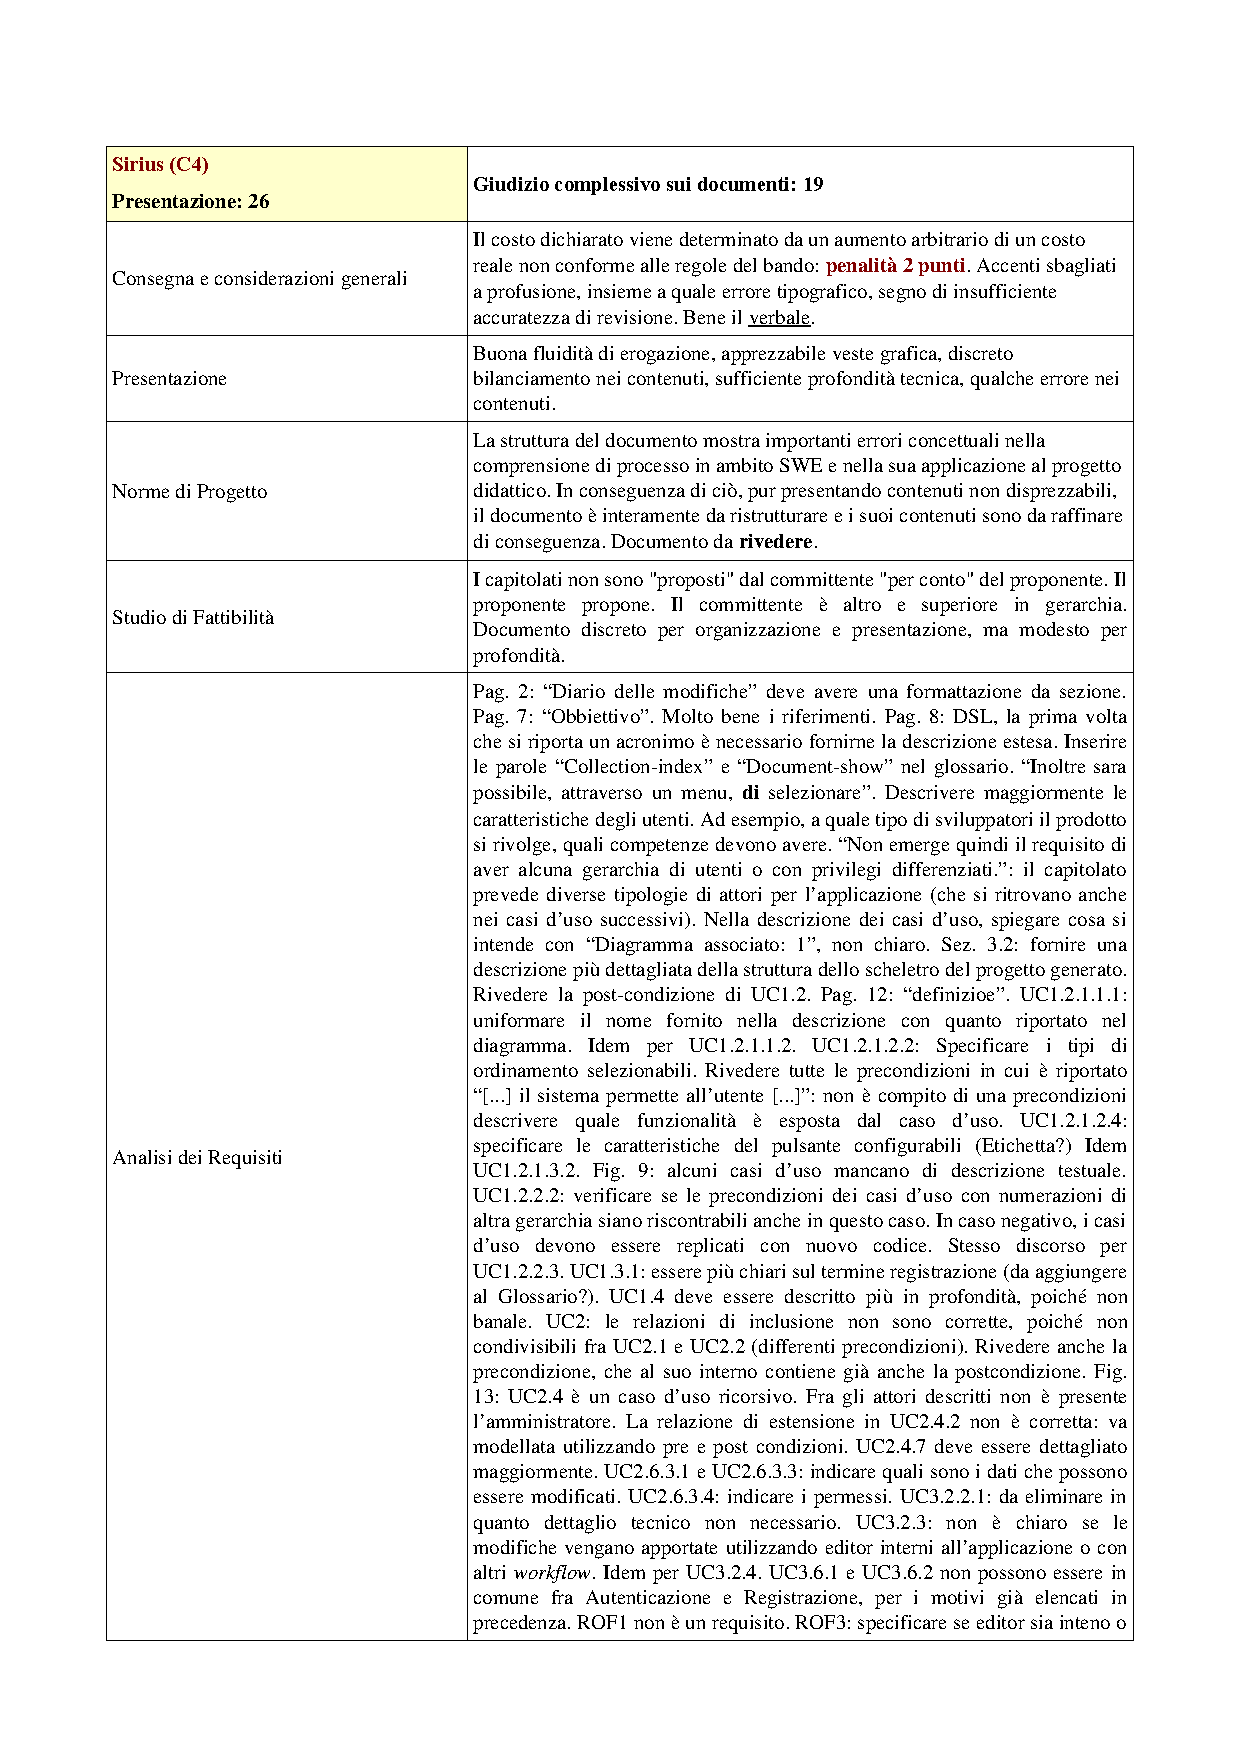
\includegraphics[scale=0.001]{img/Sirius.png}}
        \end{picture}}
	\rhead{\groupname}
	\chead{}
	\lfoot{\info}
	\cfoot{}
%	\rfoot{\thepage}
	\rfoot{\thepage\ / \pageref{LastPage}}
	\renewcommand{\headrulewidth}{0.3pt}
	\renewcommand{\footrulewidth}{0.3pt}
\linespread{1.2}	% valore interlinea


\fancypagestyle{romano}{
	\lhead{\setlength{\unitlength}{1mm}
        \begin{picture}(0,0)
                \put(5,0){
\includegraphics[scale=0.03]{../modello/img/sirius.png}}
        \end{picture}}
	\chead{}
	\rhead{\groupname}
	\lfoot{\info}
	\cfoot{}
	\rfoot{\thepage}
	\renewcommand{\headrulewidth}{0.3pt}
	\renewcommand{\footrulewidth}{0.3pt}
}



\hypersetup{
    colorlinks=true,linkcolor=[rgb]{0.11,0.55,0.83
    },          % colore link interni
    urlcolor=cyan           %colore link esterni
}
\definecolor{err}{rgb}{0.9,0.1,0.1}
\definecolor{rt}{rgb}{0.1,0.6,0.8}
\definecolor{grey}{rgb}{0.4,0.3,0.4}
\definecolor{mycolor}{rgb}{0.67,1,0.18}

\bibliographystyle{plain_ita}%bibliografia stile italiano

\pagenumbering{Roman}
\setlength\parindent{0pt} % sempre senza indentatura
% fine layout% layout
\begin{document}
% Prima pagina di opgni documento
\begin{titlepage}
 \begin{center}
     
\includegraphics[width=11cm]{../modello/img/sirius}\\
     \vspace{1em}
     {\LARGE \textsc{Sirius}}\\
     \vspace{2em} \hrule \vspace{2em}
     {\Large \textsc{Sequenziatore}}\\
     \vspace{8em}
     {\LARGE \LARGE \LARGE \textbf{\doctitle}}\\
     \vspace{2em}
     {\LARGE \LARGE \LARGE \textbf{Versione \lastversion }}\\
     \vspace{4em}
 \end{center}


\vskip 1.8cm
\begin{center}
\textit{Ingegneria Del Software AA 2013-2014}
\end{center}

\end{titlepage}


% pagina del titolo
\thispagestyle{romano}
\noindent\begin{Large}\textbf{Informazioni documento}\end{Large}\\
\begin{center}
\begin{tabular}{ll}
\hline\\
Titolo documento: & Analisi dei requisiti\\
Data creazione: & 1 Febbraio 2014\\
Versione attuale: & \lastversion\\
Utilizzo: & Esterno\\
Nome file:& \AnalisiDeiRequisiti{}\\
Redazione: & Botter Marco\\
& Giachin Vanni\\
& Marcomin Gabriele\\
Verifica: & Seresin Davide\\
Approvazione: & Quaglio Davide\\
Distribuito da:& Sirius\\
Destinato a: & Prof. Vardanega Tullio\\
			 & Prof. Cardin Riccardo\\
			 & Zucchetti S.p.A.
\end{tabular}
\end{center}
\vskip 1.5cm
%\noindent {\begin{LARGE}\textbf{Sommario}\end{LARGE}}\\
\noindent\begin{Large}\textbf{Sommario}\end{Large}\\

\noindent Risultato dello studio di fattibilità della ditta Sirius per il capitolato C04 Seq\\
\newpage
\pagestyle{romano}
\noindent\begin{Large}\textbf{Diario delle modifiche}\end{Large}\\
\\
%Inserire in testa ogni nuova versione\\
\begin{small}
\begin{tabular}{|c|p{1.8cm}|p{2.8cm}|p{2.8cm}|p{3.5cm}|}
\hline
Versione & Data & Autore & Ruolo & Descrizione \\
\hline
\hline
1.0.0 & 2014-03-05 & 
\textit{Quaglio Davide} &
\textit{Responsabile} &  Approvazione del documento\\
\hline
0.1.0 & 2014-02-13 & 
\textit{Botter Marco} &
\textit{Verificatore} &  Verifica del documento\\
\hline
0.0.2 & 2014-02-11 & 
\textit{Seresin Davide} &
\textit{Analista} &  Aggiunte e modifiche\\
\hline
0.0.1 & 2014-02-09 & 
\textit{Santangelo Davide} &
\textit{Analista} &  Creato lo scheletro del documento\\
\hline
\end{tabular}\\
\end{small}


\newpage
\pagestyle{romano}

\tableofcontents %sommario
\pagestyle{romano}



\newpage
\pagestyle{plain}
<<<<<<< HEAD

\setlength\parindent{0pt}
=======
\pagenumbering{arabic}%numeri di pagina arabi
\section{Introduzione}
\subsection{Glossario}
Al fine di facilitare la compresione del seguente documento, ed in generale di ogni documento che verrà forinto da parte del team Sirius, è stato creato appositamente un glossario (\textit{Glossario v1.2.0.pdf}) contenente la definizione dei termini più complessi o di quelli che necessitano un approfondimento.
$ Questi vocaboli sono contrassegnati in ogni documento dal pedice G (_G).
$ \subsection{Scopo del documento}
Tale documento si prefigge lo scopo di riassumere la discussione e le scelte che hanno portato il team Sirius alla scelta del capitolato \textit{C04 Sequenziatore}.
\subsection{Fonti}
\begin{itemize}
\item Capitolato d'appalto C1:\textit{ MaaP: MongoDB as an admin Platform} \\
\url{http://www.math.unipd.it/ ~ tullio/IS-1/2013/Progetto/C1.pdf;}
\item  Capitolato d'appalto C2: \textit{RING: Residue Interaction Network Generator}\\
\url{http://www.math.unipd.it/ ~ tullio/IS-1/2013/Progetto/C2.pdf;}
\item  Capitolato d'appalto C3: \textit{Romeo: Medical Imaging Cluster Analysis Tool}\\
\url{http://www.math.unipd.it/ ~ tullio/IS-1/2013/Progetto/C3.pdf;}
\item Capitolato d'appalto C4: \textit{Seq: Gestore di processi sequenziali con esecuzione da smartphone}\\
\url{http://www.math.unipd.it/ ~ tullio/IS-1/2013/Progetto/C4.pdf;}
\item Capitolato d'appalto C5:  \textit{SGAD: Social Game con Architettura Distribuita}
\url{http://www.math.unipd.it/ ~ tullio/IS-1/2013/Progetto/C5.pdf.}
\end{itemize}
\section{Capitolato C4 Seq}
\subsection{Analisi}
\subsection{Introduzione}
Il capitolato proposto dai committenti Prof. Vardanega e Prof. Cardin per conto della Zucchetti S.P.A prevede la realizzazione di un Sequenziatore, inteso come strumento per la verifica del compimento di passi astratti.
\subsubsection{Studio dei fattori favorevoli}
\begin{itemize}
\item Gli strumenti da utilizzare (HTML5, javascript, database) per lo svolgimento del progetto sono di forte interesse da parte di tutti i componenti del gruppo;
\item Lo studio del concetto di \textbf{workflow}, della creazione, validazione, verifica di passi \textbf{step by step} dipendenti, considerando la sua relazione con la gestione del lavoro in team;
\item Le conoscenze di base del team Sirius sulla tecnologia mobile sono in parte già acquisite da 3 membri su 6;
\item La libertà concessa dal capitolato permette di spaziare maggiormente con le idee, sia riguardo la sua implementazione che riguardo possibili features aggiuntive.
\end{itemize}
\subsubsection{Studio delle criticità}
\begin{itemize}
\item Il capitolato lascia ampia scelta riguardo le tecnologie da utilizzare, questa libertà potrà causare futuri conflitti nelle scelte progettuali;
\item Essendo HTML5 uno standard non completamente supportato, si corre il rischio di scrivere codice vincolato solamente all'utilizzo dei broswer in grado di supportarlo;
\item Si intravede una difficoltà nel concretizzare l'idea astratta di sequenziatore, questo a causa del fatto che i requisiti e le funzionalità del programma da implementare sono parse parzialmente vaghe nel capitolato.
\end{itemize}

\subsection{Analisi del mercato}
Dal capitolato si evince che il prodotto andrà ad inserirsi all'interno del mercato del mondo mobile, mercato tutt'ora in espansione anche se in parte già saturo. Sviluppare quindi un applicazione multipiattaforma grazie ad HTML5 garantirebbe ad essa una maggior probabilità di essere conosciuta.
Essendo inoltre molto ampia la tipologia di utilizzi che uno strumento come il sequenziatore può fornire, si intuisce che gli utenti potenzialmente interessati sono innumerevoli.

\subsection{Conclusioni}
 Alla luce di tutto ciò, creare una conoscenza di base ed una piccola esperienza sull'utilizzo degli strumenti sopracitati potrebbe rivelarsi in futuro un'opportunità, nonchè un punto di partenza, per la nostra carriera lavorativa. Un esempio è la programmazione java lato server, base indispensabile, che abbiamo già avuto modo di conoscere tramite il corso di studi e che sicuramente approfondiremo durante lo sviluppo del progetto. Inoltre, il tema proposto non richiede conoscenze particolari che divergono dall'ambiente informatico, portandoci quindi a concludere che sviluppare il capitolato: \textit{Seq: Gestore di processi sequenziali con esecuzione da smartphone}, era una scelta condivisa da tutti i membri del gruppo. \\

\section{Altri capitolati}
\subsection{Premessa}
Di seguito riportiamo l'elenco dei requisiti rilevati dalla lettura dei capitolati e una breve analisi che evidenzia le motivazioni che ci hanno portato ad escluderli.\\
\subsection{C1 MaaP Analisi}
Elenco generico dei requisiti richiesti dal capitolato:
\begin{itemize} 
\item Utilizzo di strumenti open source;
\item Gestione di database, e conoscenza di database non relazionali;
\item Conoscenza di base del \textbf{mondo business}, per creare report adatti alla categoria dell'utilizzatore finale;
\item Linguaggio di programmazione per la gestione dei dati Javascript;
\item Il capitolato prevede la realizzazione lato server, lato client, creazione dinamica di pagine web, modulo per l'interfacciamento al database e recupero dei dati.
\end{itemize}
Dall' analisi del capitolato esso risulta essere un progetto interessante per quanto riguarda la strumentazione da utilizzare, ma allo stesso tempo le risorse del team Sirius non sarebbero adatte alla mole di lavoro richiesta. Dal nostro studio possiamo prevedere che le ore di ricerca di strumenti open source, creazione di conoscenze riguardanti database non relazionali, unite alla realizzazione di tutto il pacchetto richiesto dal cliente, avrebbero portato ad un sovraccarico di lavoro.
\\
\subsection{C2 Ring Analisi}
Elenco generico dei requisiti richiesti dal capitolato:
\begin{itemize} 
\item Conoscenze di biologia;
\item Implementare algoritmi che richiamano la teoria dei grafi;
\item Linguaggio di programmazione C++ o Java;
\item Interfacciamento con software specifici inerente il settore di utilizzo.
\end{itemize}
Il capitolato presentato riguarda la realizzazione di un'interessante applicativo per la gestione delle strutture proteiche. La scelta di declinare questo capitolato è stata dettata principalmente dalle nulle conoscenze di biologia che risultano fondamentali per lo sviluppo del progetto.\\
\subsection{C3 Romeo Analisi}
Elenco generico dei requisiti richiesti dal capitolato:
\begin{itemize} 
\item Elaborazione immagini sia 2D che 3D;
\item Algoritmi di estrazione dati da immagini;
\item Studio del protocollo di elaborazione dati.
\end{itemize}
L'utilizzo di strumenti informatici come ausilio delle strutture mediche presenti è sicuramente un aspetto interessante da sviluppare. Nel capitolato sopracitato gli strumenti informatici avrebbero coadiuvato gli esami clinici restituendo un risultato sotto forma di immagine, questa sarebbe stata il punto di partenza per la prima analisi automatizzata atta ad evidenziare determinate specifiche. Le elaborazioni anche se elementari di immagini richiedono tempo ed algoritmi ottimizzati in quanto la mole di dati da elaborare potrebbe essere molto elevata. Lo studio e la ricerca di questi algoritmi di elaborazione avrebbe richiesto troppo tempo per la nostra tipologia di gruppo. Anche se le conoscenze mediche sarebbero passate in secondo piano in quanto la richiesta prevedeva lo sviluppo di un solo algoritmo di elaborazione, abbiamo deciso di declinare questo capitolato.   \\
\subsection{C5 Sgad Analisi}
Elenco generico dei requisiti richiesti dal capitolato:
\begin{itemize} 
\item Architettura distribuita;
\item Conoscenze di grafica per la creazione di gioco;
\item Vincoli precisi riguardo i giocatori;
\item Utilizzo database.
\end{itemize}
Lo studio di architetture distribuite su richieste del client avrebbe portato ogni componente del gruppo ad acquisire conoscenze importanti circa gli aspetti analizzati e specifiche competenze che solo dopo un approfondito studio si potrebbero acquisire. Nonostante questo, la realizzazione di un'architettura di questo tipo sarebbe stata molto dispendiosa in merito a tempo che sarebbe stato sottratto alla realizzazione della parte grafica su web. Quest'ultima ragione ha portato ad escludere il suddetto capitolato.\\
>>>>>>> d7eb01229571ba80af69ff5f85a34e7474917217


\pagenumbering{arabic}%numeri di pagina arabi
\setcounter{page}{1}

\section{Introduzione}

\subsection{Scopo del documento}
Il documento definisce le norme, convenzioni e formalismi  che ciascun membro del gruppo \gruppo{} deve adottare durante l'intera produzione del software \progetto{}.
In particolare tali norme regolamentano i seguenti aspetti:

\begin{itemize}
\item Organizzazione tra i membri del gruppo;
\item Stili e convenzioni nella redazione dei documenti;
\item Metodi operativi e convenzioni nelle fasi di progetto;
\item Ambiente di lavoro.
\end{itemize}

\subsection{Glossario}
Al fine di facilitare la comprensione dei documenti, i termini tecnici, di dominio e gli acronimi, sono definiti in dettaglio nel documento GLOSSARIO.\\
Tali termini sono contrassegnati dal simbolo \ped{$\vert$G$\vert$} che li segue.

\section{Processo di documentazione}
\subsection{Template}
Ogni documento dovrà essere generato includendo il \textit{template} \LaTeX presente nella cartella "Modello".
Questo modello è stato creato prima dell'inizio della redazione di ogni altro documento del team \gruppo{}, la sua modifica può avvenire solo presentando all'\textit{Amministratore} una richiesta formale, allegandone la motivazione ed il tipo di modifica richiesta. Se l'\textit{Amministratore} riterrà opportuno effettuare il cambiamento, prima di apportare la modifica dovrà avvertire l'intero team al fine di evitare disguidi.

\subsection{Classificazione documenti}
\subsubsection{Documenti formali}
Sono catalogati come formali tutti i documenti approvati dal \textit{Responsabile di Progetto}, ovvero i documenti ritenuti pronti per essere visionati dal committente. Tali documenti, prima di raggiungere l'approvazione dovranno aver superato con successo la procedura di verifica e validazione riportata nel \textit{Piano di Qualifica}.
\subsubsection{Documenti informali}
Tutti i documenti che non sono stati approvati dal \textit{Responsabile di Progetto} sono da ritenersi informali, e di utilizzo esclusivamente interno. Tutti i documenti non versionati sono da ritenersi non ufficiali.

\subsection{Versionamento documenti}
Il versionamento di tutta la documentazione del gruppo \gruppo{} è stato organizzato secondo le seguenti convenzioni:
\begin{itemize}
\item Il numero di versionamento deve essere nella forma:

\begin{center}
\textbf{X}, \textbf{Y}, \textbf{Z}
\end{center}

con \textbf{X}, \textbf{Y}, \textbf{Z} numeri interi non negativi;
\item Tutti gli elementi devono salire di una sola unità alla volta.
\end{itemize}

Di seguito vengono inoltre riportati i significati che possono assumere le variazioni della versione del documento:
\begin{itemize}
\item La \textbf{X} rappresenta il numero di uscite formali del documento, ogni qual volta un documento verrà pubblicato il valore della cifra \textbf{Y} e della cifra \textbf{Z} verrà azzerato. Riportando quanto detto più precisamente:
\begin{enumerate}
\item X assumerà il valore: 1, alla \textbf{revisione dei requisiti};
\item X assumerà il valore: 2, alla \textbf{revisione di progettazione};
\item X assumerà il valore: 3, alla \textbf{revisione di qualifica};
\item X assumerà il valore: 4, alla \textbf{revisione di accettazione}.
\end{enumerate}
\item La \textbf{Y} rappresenta il numero di \textit{push} effettuati sul \textit{branch\ped{G}} \textit{master} in \textit{GitHub} (sezione 8.2.1, GitHub), ossia il numero di volte in cui sono state compiute importanti modifiche al documento. Ogni qual volta aumenterà l'indice \textbf{Y} si azzererà l'indice \textbf{Z}.
\item La \textbf{Z} rappresenta il numero di modifiche minori apportate al documento durante il suo sviluppo.
Aumenta al termine di ogni sessione di lavoro sul documento.
\end{itemize}

Ogni documento formale riporterà un diario delle modifiche contenente le trasformazioni più rilevanti che ha attraversato sotto forma tabellare.

\subsection{Struttura Documentazione}
\subsubsection{Header}
Ogni pagina esclusa la prima presenta un \textit{header} raffigurante il logo del gruppo sulla sinistra, mentre sulla destra il nome del team ed il nome del progetto.
\subsubsection{Footer}
Ogni pagina esclusa la prima presenta un \textit{footer} riportante il nome del documento corredato della versione sulla sinistra, mentre sulla destra il numero della pagina.
Per il numero di pagina delle prime quattro facciate saranno utilizzati i numeri romani, a seguire invece verranno utilizzati i numeri occidentali.
\subsubsection{Prima pagina}
La prima pagina di ogni documento conterrà:
\begin{itemize}
\item Il logo del \textit{team}, riportante la scritta \gruppo;
\item Il titolo del progetto;
\item Il nome del documento e la sua versione;
\item Il nome del corso;
\item L'anno di sviluppo del progetto;
\end{itemize}

\subsubsection{Seconda pagina}
La seconda pagina di ogni documento conterrà:
\begin{itemize}
\item  Informazioni sul documento come segue:
\begin{itemize}
\item Titolo del documento;
\item Data di creazione;
\item Versione attuale;
\item Utilizzo, che specifica se il documento è per utilizzo interno o esterno;
\item Nome file;
\item Redazione;
\item Revisione;
\item Approvazione;
\item Distribuito da, a cui seguirà il nome del gruppo.
\end{itemize}
\item Un sommario riportante una breve descrizione;
\end{itemize}

\subsubsection{Terza pagina}
La terza pagina di ogni documento conterrà:
\begin{itemize}
\item Un diario delle modifiche apportate al documento, dall'inizio fino alla versione corrente.
\end{itemize}

\subsubsection{Quarta pagina}
La quarta pagina di ogni documento ne riporterà l'indice, è possibile che l'indice si estenda per più di una singola pagina. 

\subsection{Norme tipografiche}
\subsubsection{Generali}
\begin{itemize}
\item Ogni documento deve essere in lingua italiana, altre lingue possono essere utilizzate per riferirsi a termini tecnici informatici o in situazioni che lo richiedono strettamente;

\item Ogni documento deve essere grammaticalmente, sintatticamente e semanticamente corretto, cercando di essere meno verboso possibile;

\item Utilizzare il più possibile elenchi puntati invece di lunghe frasi.

\end{itemize}
\subsubsection{Punteggiatura}
\begin{itemize}
\item Non si usa mai un punto alla fine di un titolo: di capitolo, di paragrafo, di sotto-paragrafo;

\item Ogni elemento di un elenco puntato termina con un punto e virgola, se è l'ultimo elemento con un punto;

\item Prima di ogni segno di punteggiatura non va mai messo uno spazio bianco, dopo invece lo spazio bianco va messo sempre;


\item Il testo racchiuso tra parentesi non deve aprirsi o chiudersi con un carattere di spaziatura ne terminare con un carattere di punteggiatura.

\end{itemize}
\subsubsection{Ortografia}

\begin{itemize}

\item Le lettere maiuscole vanno poste solo all'inizio di ogni elemento di un elenco puntato e dove lo prevede l'ortografia italiana (all'inizio di un periodo o dopo un segno di punteggiatura forte, cioè dopo il punto fermo, i puntini di sospensione, il punto esclamativo ed il punto interrogativo). È inoltre utilizzata l'iniziale maiuscola nel nome del team, del progetto, dei documenti, dei ruoli di progetto.


\end{itemize}

\subsubsection{Stile}
\begin{itemize}
\item Se si devono elencare delle di istruzioni in serie o una divisione in paragrafi e sotto-paragrafi è necessario utilizzare un elenco numerato, altrimenti è preferibile un elenco puntato;

\item Il primo livello di profondità degli elenchi puntati è contrassegnato da un pallino nero pieno, il secondo da un trattino, il terzo da un asterisco;

\item Le date dovranno essere espresse nella forma \textbf{aaaa-mm-gg} secondo lo standard  \ped{G}\textbf{ISO G 8601:2004};

\item Gli orari dovranno essere espressi nella forma \textbf{hh:mm} secondo lo standard \textbf{ISO G 8601:2004};

\item \textbf{URL} ed indirizzi mail dovrano essere preceduto dal comando \LaTeX \verb+ \+url;

\item Ogni prima (e possibilmente anche successiva) occorrenza di una parola presente sul \textit{Glossario} sarà seguita da pedice \ped{G}.

\item Stile di testo:

\begin{itemize}

\item Il corsivo deve essere utilizzato obbligatoriamente nelle citazioni, per il nome delle figure di rilievo (es. \textit{committente}, \textit{Responsabile di Progetto}) e per il nome dei documenti (es. \textit{Analisi dei requisiti}), mentre a discrezione del redattore per termini stranieri in modo da evidenziarli;

\item il grassetto deve essere utilizzato per evidenziare (se si reputa necessario) le parole chiave ed i passaggi particolarmente rilevanti.

\end{itemize}

\end{itemize}
\subsection{Calcolo indice di Gulpease}
In ogni documento redatto il verificatore dovrà calcolare l'indice di Gulpease, ossia il valore di leggibilità del documento.
Per raggiungere il seguente scopo è disponibile uno \textit{script online}, reperibile al sito:\\
\\
\href{http://xoomer.virgilio.it/roberto-ricci/variabilialeatorie/esperimenti/leggibilita.htm}{http://www.xoomer.virgilio.it/roberto-ricci/variabilialeatorie/esperimenti/leggibilita.htm}
\\ \\
Questo \textit{script} già esistente è stato verificato prima di essere adottato, in modo da scongiurare il rischio di incompatibilità tra i documenti redatti e la forma che doveva avere l'input per lo \textit{script}.
Se l'indice risultante di un documento si troverà in un range compreso tra lo 0 ed il 40, sarà necessario ricercare nel testo frasi troppo lunghe e complesse per reimpostarle.


\subsection{Glossario}
Durante la stesura di un documento, ogni qual volta il redattore riterrà necessario chiarire il significato di un termine utilizzato sarà tenuto ad aggiungerlo nel \textit{glossario}.\\
Il \textit{glossario} sarà strutturato seguendo questo schema:
\begin{itemize}
\item Nel file \LaTeX ogni parola sarà contenuta nel \textbf{tag}: "elemento";
\item A seguire, andando a capo-riga, sarà riportata la descrizione del termine.
\end{itemize}
Il \textit{glossario} sarà inoltre suddiviso in due sezioni:
\begin{itemize}
\item Termini;
\item Acronimi.
\end{itemize}
Termini ed acronimi dovranno essere necessariamente elencati in ordine alfabetico, la definizione dovrà essere breve ed esplicativa, inoltre sempre la definizione non potrà iniziare con una \textbf{E accentata}.

\section{Collaborazione}

\subsection{Comunicazioni}

\subsubsection{Interne}
Le comunicazioni interne generiche tra i membri del gruppo Github si svolgono attraverso la mailing list privata (gruppo Google) e facebook.

Le comunicazioni e il coordinamento formali (issue tracking, formazione, ecc.) invece si appoggiano alla piattaforma \url{https://swesirius.teamworkpm.net}

\subsubsection{Esterne}
Le comunicazioni formali esterne avvengono attraverso l’indirizzo email: \url{swesirius@gmail.com}


\subsection{Riunioni}
Con riunioni si intende qualsiasi incontro fra Proponente / Committente e un gruppo di rappresentanza (composto da almeno la maggioranza assoluta) del gruppo di progetto.

\subsubsection{Richiesta}

La richiesta di indire una riunione esterna può essere avanzata da qualsiasi componente del gruppo; e compito del Responsabile contattare ed organizzare l'evento con l'interessato. 
Una volta pianificato con il resto del gruppo secondo i passi indicati alla sezione 3.1 con tag [Riunione Esterna].

\subsubsection{Esito}

Ad ogni incontro il Responsabile ha il compito di stilare un verbale (cap. 5.8) che evidenzia i chiarimenti emersi durante l'incontro.

\subsection{Verbali incontri}

Per Verbali degli incontri si intendono quei documenti redatti dal Responsabile di Progetto in occasione di incontri esterni ed interni.
Per tali documenti e prevista una sola stesura in quanto promemoria dell'incontro avvenuto.
Non e perciò previsto il versionamento.
I Verbali degli incontri devono essere denominati secondo il seguente criterio:

\begin{center}
Verbale\{tipo incontro\}\{data incontro\}
\end{center}

\begin{itemize}
\item tipo incontro: indica il tipo di incontro e I (interno) o E (esterno);
\item data incontro: indica la data in cui  e stato tenuto l'incontro seguendo il formato.
\end{itemize}
  
  
La prima pagina di ogni verbale deve obbligatoriamente contenere i seguenti campi, nell'ordine indicato:

\begin{itemize}
\item data;
\item luogo: espresso nel formato;
\item ora di ritrovo: espressa nel formato;
\item Ora dell'incontro: fhhg:fmmg;
\item Durata dell'incontro: fxg min;
\item partecipanti interni: lista degli appartenenti Sirius presenti all'incontro;
\item partecipanti esterni: rappresentanti della ditta/e per ogni partecipante indicare il campo ruolo che rappresenta il ruolo assunto all'interno dell'azienda a cui fanno capo; nel caso il partecipante sia il Committente, il campo viene compilato con Committente;
\item contenuto: la decisione del formato  e lasciata al Responsabile di Progetto, il quale adotta lo stile più consono in base al tipo di incontro svolto;
\item firme: devono essere comprese quelle di tutti i partecipanti del gruppo Sirius a conferma della presa visione del documento.
\end{itemize}



\section{Requisiti}
Le convenzioni utilizzate per l'identificazione e la definizione dei requisiti sono riportate nel documento \NormeDiProgetto{}. 
\subsection{Requisiti funzionali}
\subsubsection{Ambito utente}
\LTXtable{\textwidth}{RequisitiUtente.tex}
\subsubsection{Ambito amministratore}
\LTXtable{\textwidth}{RequisitiAmministratore.tex}
\subsection{Requisiti di qualità}
\LTXtable{\textwidth}{RequisitiQualita.tex}
\subsection{Requisiti di vincolo}
\LTXtable{\textwidth}{RequisitiVincolo.tex} 

\section{Ambiente di lavoro}

\subsection{Gestione di progetto}
Il software utilizzato per la gestione di progetto è Teamwork (\href{http://www.teamwork.com}{www.teamwork.com}), che fornisce le seguenti funzionalità:

\begin{itemize}
\item Creazione di ticket, milestone e liste di attività;
\item Gestione dei ruoli;
\item Generazione di grafici Gantt;
\item Monitoraggio dei tempi;
\item Registro dei rischi.
\end{itemize}

\subsection{Versionamento}
Lo strumento scelto per il versionamento è Git \dots

\end{document}